% Grafo de fatores do BA local do VO (janela deslizante, BA.py).
% Compilar sozinho: pdflatex grafo_ba_local.tex
% Na dissertação: \usepackage{standalone} + \includestandalone[width=\linewidth]{figuras/grafo_ba_local}
\documentclass[tikz,border=4pt]{standalone}
\usepackage[T1]{fontenc}
\usepackage[utf8]{inputenc}
\usepackage{amsmath,amssymb,bm}
\usetikzlibrary{calc}

\definecolor{cReproj}{HTML}{2A78D6}
\definecolor{cPrior}{HTML}{0B0B0B}
\definecolor{cOdomVO}{HTML}{1BAF7A}
\definecolor{cLmPrior}{HTML}{EB6834}

\begin{document}
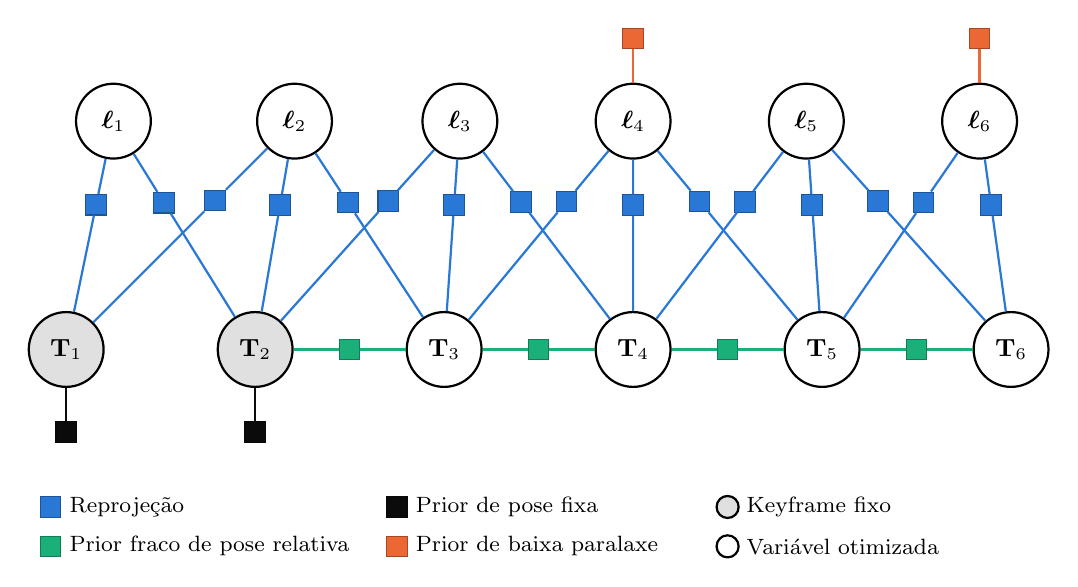
\begin{tikzpicture}[
    font=\small,
    var/.style={circle, draw, thick, minimum size=9.5mm, inner sep=0pt},
    fixo/.style={var, fill=black!12},
    fat/.style={rectangle, fill=#1, draw=#1!70!black, minimum size=2.6mm, inner sep=0pt},
    lig/.style={draw=#1, line width=0.8pt},
    leg/.style={font=\footnotesize, anchor=west, inner sep=1pt},
  ]

  % ---- variáveis: 6 keyframes na janela (2 mais antigos fixos) e 6 landmarks
  \foreach \k in {1,...,6} {
    \pgfmathsetmacro\x{2.4*(\k-1)}
    \ifnum\k<3 \node[fixo] (T\k) at (\x,0) {$\mathbf{T}_{\k}$};
    \else      \node[var]  (T\k) at (\x,0) {$\mathbf{T}_{\k}$}; \fi
  }
  \foreach \k/\x in {1/0.6, 2/2.9, 3/5.0, 4/7.2, 5/9.4, 6/11.6}
    \node[var] (l\k) at (\x,2.9) {$\bm{\ell}_{\k}$};

  % ---- fatores de reprojeção: cada landmark observado por 2 ou 3 keyframes da janela
  \foreach \l/\t in {l1/T1, l1/T2,
                     l2/T1, l2/T2, l2/T3,
                     l3/T2, l3/T3, l3/T4,
                     l4/T3, l4/T4, l4/T5,
                     l5/T4, l5/T5, l5/T6,
                     l6/T5, l6/T6} {
    \path (\l) -- (\t) node[pos=0.3, fat=cReproj] (r-\l-\t) {};
    \draw[lig=cReproj] (\l) -- (r-\l-\t) -- (\t);
  }

  % ---- prior em landmarks de baixa paralaxe (unário)
  \foreach \l in {l4, l6} {
    \node[fat=cLmPrior] (p\l) at ($(\l)+(0,1.05)$) {};
    \draw[lig=cLmPrior] (\l) -- (p\l);
  }

  % ---- prior fraco de pose relativa (KFs consecutivos com ao menos um livre: não entre T1 e T2)
  \foreach \a/\b in {T2/T3, T3/T4, T4/T5, T5/T6} {
    \path (\a) -- (\b) node[midway, fat=cOdomVO] (o-\a-\b) {};
    \draw[lig=cOdomVO] (\a) -- (o-\a-\b) -- (\b);
  }

  % ---- prior de pose fixa nos 2 KFs mais antigos (unário)
  \foreach \t in {T1, T2} {
    \node[fat=cPrior] (p-\t) at ($(\t)+(0,-1.05)$) {};
    \draw[lig=cPrior] (\t) -- (p-\t);
  }

  % ---- legenda (3 colunas)
  \begin{scope}[shift={(-0.2,-2.0)}]
    \node[fat=cReproj]  at (0,0)       {}; \node[leg] at (0.2,0)      {Reprojeção};
    \node[fat=cOdomVO]  at (0,-0.5)    {}; \node[leg] at (0.2,-0.5)   {Prior fraco de pose relativa};
    \node[fat=cPrior]   at (4.4,0)     {}; \node[leg] at (4.6,0)      {Prior de pose fixa};
    \node[fat=cLmPrior] at (4.4,-0.5)  {}; \node[leg] at (4.6,-0.5)   {Prior de baixa paralaxe};
    \node[circle, draw, thick, fill=black!12, minimum size=2.8mm, inner sep=0pt] at (8.6,0) {};
    \node[leg] at (8.8,0) {Keyframe fixo};
    \node[circle, draw, thick, minimum size=2.8mm, inner sep=0pt] at (8.6,-0.5) {};
    \node[leg] at (8.8,-0.5) {Variável otimizada};
  \end{scope}
\end{tikzpicture}
\end{document}
